\documentclass[aspectratio=169,11pt]{beamer}

\usetheme{Madrid}
\usecolortheme{default}
\setbeamercovered{transparent}

\usepackage{graphicx}
\usepackage{amsmath}
\usepackage{amssymb}
\usepackage{booktabs}
\usepackage{tikz}
\usetikzlibrary{arrows.meta, shapes.geometric, positioning,
                fit, backgrounds, shadows.blur,
                decorations.pathreplacing, calc}

\setbeamersize{text margin left=0.6cm, text margin right=0.6cm}
\setlength{\leftmargini}{0.9em}
\setlength{\leftmarginii}{1.4em}

% ── Shared TikZ styles (mirrors DIP presentation) ─────────────────────────────
\tikzset{
  pipenode/.style={
    rectangle, rounded corners=4pt,
    minimum width=1.6cm, minimum height=0.9cm,
    text centered, font=\scriptsize\bfseries,
    draw=#1!70!black, fill=#1!30, text=#1!20!black,
    drop shadow
  },
  pipearrow/.style={-Stealth, thick, color=gray!70},
  sysbox/.style={
    rectangle, rounded corners=5pt,
    minimum width=2.8cm, minimum height=0.85cm,
    text centered, font=\scriptsize\bfseries,
    draw=#1!70!black, fill=#1!25, text=#1!20!black,
    drop shadow
  },
  flowbox/.style={
    rectangle, rounded corners=4pt,
    minimum width=3.2cm, minimum height=0.7cm,
    text centered, font=\scriptsize,
    draw=blue!50!black, fill=blue!10, text=blue!20!black
  },
  metricbox/.style={
    rectangle, rounded corners=5pt,
    minimum width=2.6cm, minimum height=1.4cm,
    text centered, font=\small\bfseries,
    draw=#1!70!black, fill=#1!20, text=#1!20!black,
    drop shadow
  },
  layernode/.style={
    rectangle, rounded corners=4pt,
    minimum width=8.8cm, minimum height=0.78cm,
    text centered, font=\scriptsize,
    draw=#1!65!black, fill=#1!18, text=#1!20!black
  },
}

\title{Brain Tumour Detection Using\\Convolutional Neural Networks}
\subtitle{CEP: Artificial Intelligence and Machine Learning Lab}
\author{%
  Muhammad Ahmad~{\small(FA23-BCE-113)}\\[2pt]
  Uzair~{\small(FA23-BCE-098)}%
}
\date{\today}
\institute{Computer Engineering Department\\COMSATS University Islamabad -- Lahore Campus}

\begin{document}

% ── Custom footer ─────────────────────────────────────────────────────────────
\setbeamertemplate{footline}{%
  \leavevmode%
  \hbox{%
    \begin{beamercolorbox}[wd=0.20\paperwidth, ht=2.5ex, dp=1.5ex,
                           leftskip=0.3cm]{author in head/foot}%
    \end{beamercolorbox}%
    \begin{beamercolorbox}[wd=0.60\paperwidth, ht=2.5ex, dp=1.5ex,
                           center]{title in head/foot}%
      \usebeamerfont{title in head/foot}%
      \textbf{Brain Tumour Detection --- CNN Pipeline}%
    \end{beamercolorbox}%
    \begin{beamercolorbox}[wd=0.20\paperwidth, ht=2.5ex, dp=1.5ex,
                           rightskip=0.3cm, right]{date in head/foot}%
      \usebeamerfont{date in head/foot}%
      \insertframenumber{} / \inserttotalframenumber%
    \end{beamercolorbox}%
  }%
  \vskip0pt%
}

% ===== TITLE =====
\begin{frame}
    \titlepage
\end{frame}

% ===== OUTLINE =====
\begin{frame}{Outline}
    \tableofcontents
\end{frame}

% ===========================================================================
\section{Introduction}
% ===========================================================================

\begin{frame}{Problem Statement}
    \begin{itemize}\setlength\itemsep{5pt}
        \item \textbf{Challenge:} Brain tumours are among the most life-threatening neurological disorders
        \item Manual MRI interpretation is time-consuming and requires specialist radiologists
        \item Human analysis is prone to fatigue-induced errors and inter-observer variability
        \item Limited radiologist access in resource-constrained and rural regions
        \item \textbf{Solution:} Deep CNN-based automated binary classification of brain MRI scans
    \end{itemize}
    \vspace{0.35cm}
    \begin{center}
        \small\textit{Objective: Train a robust CNN to classify brain MRI scans as%
        \textbf{ Normal} or \textbf{Tumour-Positive} with clinical-grade sensitivity}
    \end{center}
\end{frame}

\begin{frame}{Key Objectives}
    \begin{columns}[T]
        \column{0.48\textwidth}
        \textbf{Primary Goals:}
        \begin{itemize}\setlength\itemsep{3pt}
            \item Binary classification of MRI scans
            \item Maximise sensitivity (minimise false negatives)
            \item Learn discriminative spatial features
            \item Enable real-time inference via API
            \item Support downstream DIP pipeline
        \end{itemize}
        \column{0.48\textwidth}
        \textbf{Technical Requirements:}
        \begin{itemize}\setlength\itemsep{3pt}
            \item Four-stage CNN architecture
            \item Data augmentation for generalisation
            \item Quantitative metric evaluation
            \item PCA feature space visualisation
            \item FastAPI deployment-ready export
        \end{itemize}
    \end{columns}
    \vspace{0.45cm}
    \centering
    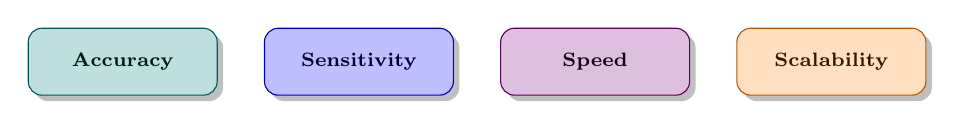
\begin{tikzpicture}
      \node[sysbox=teal,   minimum width=2.4cm] at (0,0)   {Accuracy};
      \node[sysbox=blue,   minimum width=2.4cm] at (3.0,0) {Sensitivity};
      \node[sysbox=violet, minimum width=2.4cm] at (6.0,0) {Speed};
      \node[sysbox=orange, minimum width=2.4cm] at (9.0,0) {Scalability};
    \end{tikzpicture}
\end{frame}

% ===========================================================================
\section{Dataset}
% ===========================================================================

\begin{frame}{Dataset Overview}
    \begin{columns}[T]
        \column{0.50\textwidth}
        \textbf{Brain Tumour MRI Dataset:}
        \begin{itemize}\setlength\itemsep{4pt}
            \item 255 grayscale MRI scan images
            \item Two classes: Normal and Tumour
            \item Resized to $128 \times 128$ pixels
            \item Label mode: \texttt{binary}
            \item 80/20 train--validation split
        \end{itemize}
        \vspace{0.3cm}
        \textbf{Loading Method:}\\[3pt]
        {\scriptsize\texttt{tf.keras.utils.image\_dataset\_from\\\_directory()} with \texttt{validation\_split=0.20}}

        \column{0.46\textwidth}
        \centering\vspace{0.1cm}
        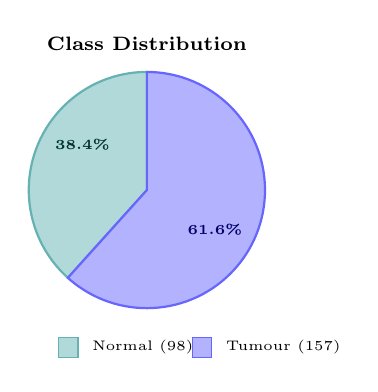
\begin{tikzpicture}
          % Pie-chart approximation using arcs
          \fill[teal!30, draw=teal!60, thick]
            (0,0) -- (90:1.5cm) arc[start angle=90, end angle=228, radius=1.5cm] -- cycle;
          \fill[blue!30, draw=blue!60, thick]
            (0,0) -- (228:1.5cm) arc[start angle=228, end angle=450, radius=1.5cm] -- cycle;
          \node[font=\tiny\bfseries, text=teal!40!black]  at (145:1.0cm) {38.4\%};
          \node[font=\tiny\bfseries, text=blue!40!black]  at (330:1.0cm) {61.6\%};
          \node[font=\tiny, below=1.75cm] at (0,0) {};
          % Legend
          \node[rectangle, fill=teal!30, draw=teal!60,
                minimum width=0.25cm, minimum height=0.25cm]
               (lt) at (-1.0,-2.0){};
          \node[right=0.05cm of lt, font=\tiny]{Normal (98)};
          \node[rectangle, fill=blue!30, draw=blue!60,
                minimum width=0.25cm, minimum height=0.25cm]
               (lb) at (0.7,-2.0){};
          \node[right=0.05cm of lb, font=\tiny]{Tumour (157)};
          \node[font=\scriptsize\bfseries, above=1.65cm] at (0,0) {Class Distribution};
        \end{tikzpicture}
    \end{columns}
\end{frame}

\begin{frame}{Data Augmentation Strategy}
    \centering
    \vspace{0.1cm}
    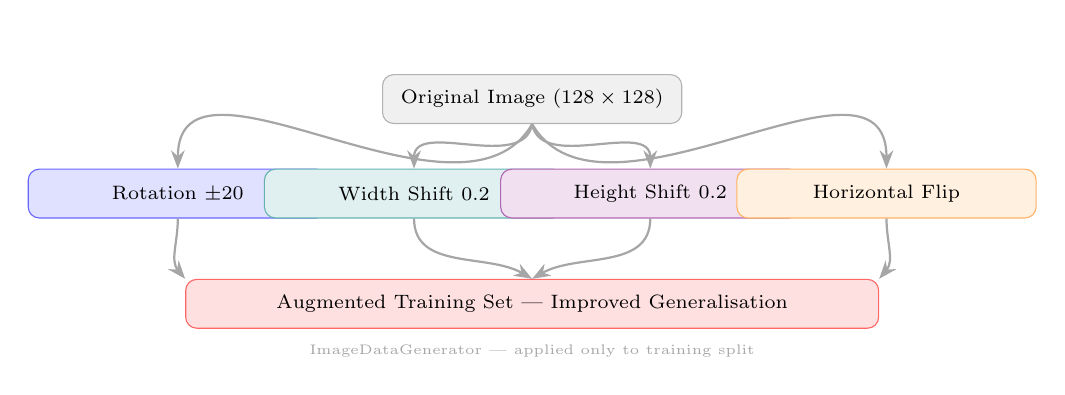
\begin{tikzpicture}[
        every node/.style={font=\scriptsize},
        aug/.style={
          rectangle, rounded corners=4pt,
          minimum width=3.8cm, minimum height=0.62cm,
          text centered, draw=#1!60, fill=#1!12
        }
      ]
      \node[aug=gray](orig) at (0, 0)    {Original Image ($128\times128$)};

      \node[aug=blue]  (rot)  at (-4.5,-1.2) {Rotation $\pm 20°$};
      \node[aug=teal]  (wsh)  at (-1.5,-1.2) {Width Shift 0.2};
      \node[aug=violet](hsh)  at ( 1.5,-1.2) {Height Shift 0.2};
      \node[aug=orange](hfl)  at ( 4.5,-1.2) {Horizontal Flip};

      \draw[pipearrow] (orig.south) to[out=240,in=90] (rot.north);
      \draw[pipearrow] (orig.south) to[out=260,in=90] (wsh.north);
      \draw[pipearrow] (orig.south) to[out=280,in=90] (hsh.north);
      \draw[pipearrow] (orig.south) to[out=300,in=90] (hfl.north);

      \node[aug=red, minimum width=8.8cm](aug) at (0,-2.6)
           {Augmented Training Set --- Improved Generalisation};

      \draw[pipearrow] (rot.south)  to[out=270,in=130] (aug.north west);
      \draw[pipearrow] (wsh.south)  to[out=270,in=150] (aug.north);
      \draw[pipearrow] (hsh.south)  to[out=270,in=30]  (aug.north);
      \draw[pipearrow] (hfl.south)  to[out=270,in=50]  (aug.north east);

      \node[font=\tiny, text=gray!70, below=0.08cm of aug]
           {ImageDataGenerator --- applied only to training split};
    \end{tikzpicture}
\end{frame}

% ===========================================================================
\section{CNN Architecture}
% ===========================================================================

\begin{frame}{Four-Stage CNN Architecture}
  \centering
  \vspace{0.1cm}
  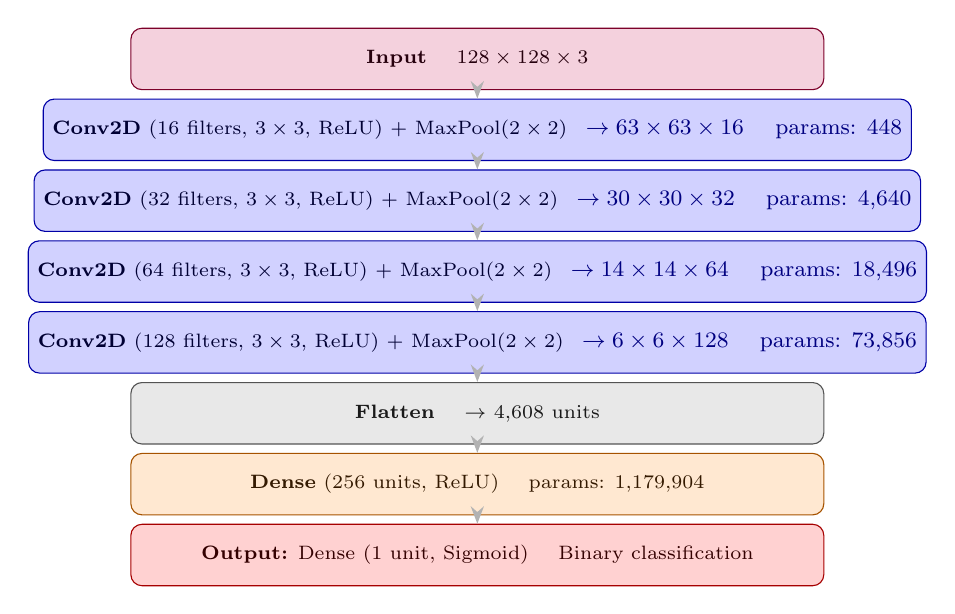
\begin{tikzpicture}[
      every node/.style={font=\scriptsize},
      arr/.style={-{Stealth[length=2.2mm]}, line width=0.9pt, draw=gray!60}
    ]
    \node[layernode=purple] (inp) at (0, 0.00)
         {\textbf{Input} \quad $128 \times 128 \times 3$};

    \node[layernode=blue]   (b1)  at (0,-0.90)
         {\textbf{Conv2D} (16 filters, $3\times3$, ReLU) $+$ MaxPool($2\times2$)
          \enspace{\color{blue!50!black}\footnotesize $\to 63\times63\times16$ \quad params: 448}};

    \node[layernode=blue]   (b2)  at (0,-1.80)
         {\textbf{Conv2D} (32 filters, $3\times3$, ReLU) $+$ MaxPool($2\times2$)
          \enspace{\color{blue!50!black}\footnotesize $\to 30\times30\times32$ \quad params: 4{,}640}};

    \node[layernode=blue]   (b3)  at (0,-2.70)
         {\textbf{Conv2D} (64 filters, $3\times3$, ReLU) $+$ MaxPool($2\times2$)
          \enspace{\color{blue!50!black}\footnotesize $\to 14\times14\times64$ \quad params: 18{,}496}};

    \node[layernode=blue]   (b4)  at (0,-3.60)
         {\textbf{Conv2D} (128 filters, $3\times3$, ReLU) $+$ MaxPool($2\times2$)
          \enspace{\color{blue!50!black}\footnotesize $\to 6\times6\times128$ \quad params: 73{,}856}};

    \node[layernode=gray]   (fl)  at (0,-4.50)
         {\textbf{Flatten} \quad $\to$ 4{,}608 units};

    \node[layernode=orange] (d1)  at (0,-5.40)
         {\textbf{Dense} (256 units, ReLU) \quad params: 1{,}179{,}904};

    \node[layernode=red]    (out) at (0,-6.30)
         {\textbf{Output:} Dense (1 unit, Sigmoid) \quad Binary classification};

    \foreach \a/\b in {inp/b1, b1/b2, b2/b3, b3/b4, b4/fl, fl/d1, d1/out}
      \draw[arr] (\a.south)--(\b.north);

  \end{tikzpicture}

  \vspace{4pt}
  {\scriptsize
  \begin{tabular}{@{}ll@{\enspace}ll@{\enspace}ll@{\enspace}ll@{}}
    \raisebox{2pt}{\colorbox{purple!18}{\phantom{X}}} & Input &
    \raisebox{2pt}{\colorbox{blue!18}{\phantom{X}}}   & Conv+Pool &
    \raisebox{2pt}{\colorbox{gray!20}{\phantom{X}}}   & Flatten &
    \raisebox{2pt}{\colorbox{orange!18}{\phantom{X}}} & Dense (hidden) \quad
    \raisebox{2pt}{\colorbox{red!18}{\phantom{X}}}      Output
  \end{tabular}}
\end{frame}

\begin{frame}{Layer-by-Layer Summary}
  \centering
  \renewcommand{\arraystretch}{1.25}
  {\small
  \begin{tabular}{|l|c|c|c|}
  \hline
  \rowcolor{black}
  \textcolor{white}{\textbf{Layer}} &
  \textcolor{white}{\textbf{Output Shape}} &
  \textcolor{white}{\textbf{Params}} &
  \textcolor{white}{\textbf{Activation}} \\
  \hline
  Input ($128\times128\times3$)    & (None,128,128,3)   & ---           & --- \\
  \hline
  Conv2D (16, $3\times3$)          & (None,126,126,16)  & 448           & ReLU \\
  MaxPool ($2\times2$)             & (None, 63, 63, 16) & 0             & --- \\
  \hline
  Conv2D (32, $3\times3$)          & (None, 61, 61, 32) & 4{,}640       & ReLU \\
  MaxPool ($2\times2$)             & (None, 30, 30, 32) & 0             & --- \\
  \hline
  Conv2D (64, $3\times3$)          & (None, 28, 28, 64) & 18{,}496      & ReLU \\
  MaxPool ($2\times2$)             & (None, 14, 14, 64) & 0             & --- \\
  \hline
  Conv2D (128, $3\times3$)         & (None, 12, 12,128) & 73{,}856      & ReLU \\
  MaxPool ($2\times2$)             & (None,  6,  6,128) & 0             & --- \\
  \hline
  Flatten                          & (None, 4{,}608)    & 0             & --- \\
  Dense (256)                      & (None, 256)        & 1{,}179{,}904 & ReLU \\
  Dense (1) --- Output             & (None, 1)          & 257           & Sigmoid \\
  \hline
  \rowcolor{gray!15}
  \textbf{Total Parameters}        & \multicolumn{3}{c|}{\textbf{1{,}277{,}601 \quad (4.87 MB)}} \\
  \hline
  \end{tabular}}
\end{frame}

% ===========================================================================
\section{Training Procedure}
% ===========================================================================

\begin{frame}{Training Configuration}
    \begin{columns}[T]
        \column{0.50\textwidth}
        \textbf{Hyperparameters:}
        \begin{itemize}\setlength\itemsep{4pt}
            \item \textbf{Optimizer:} Adam ($lr = 0.001$)
            \item \textbf{Loss:} BinaryCrossentropy
            \item \textbf{Metric:} Accuracy
            \item \textbf{Epochs:} 10 (EarlyStopping, patience = 5)
            \item \textbf{Batch Size:} 32
            \item \textbf{Val Split:} 20\,\% (51 images)
        \end{itemize}
        \column{0.46\textwidth}
        \centering\vspace{0.1cm}
        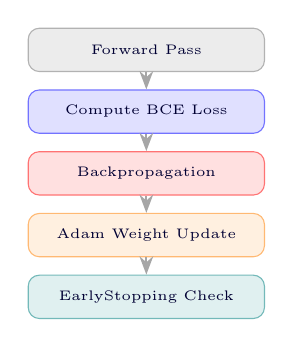
\begin{tikzpicture}[node distance=0.3cm]
          \node[flowbox, fill=gray!15, draw=gray!60,
                minimum width=3.0cm, minimum height=0.55cm,
                font=\tiny](fw){Forward Pass};
          \node[flowbox, fill=blue!12, draw=blue!55,
                minimum width=3.0cm, minimum height=0.55cm,
                font=\tiny, below=0.22cm of fw](loss){Compute BCE Loss};
          \node[flowbox, fill=red!12, draw=red!55,
                minimum width=3.0cm, minimum height=0.55cm,
                font=\tiny, below=0.22cm of loss](bk){Backpropagation};
          \node[flowbox, fill=orange!12, draw=orange!55,
                minimum width=3.0cm, minimum height=0.55cm,
                font=\tiny, below=0.22cm of bk](up){Adam Weight Update};
          \node[flowbox, fill=teal!12, draw=teal!55,
                minimum width=3.0cm, minimum height=0.55cm,
                font=\tiny, below=0.22cm of up](chk){EarlyStopping Check};
          \draw[pipearrow](fw.south)--(loss.north);
          \draw[pipearrow](loss.south)--(bk.north);
          \draw[pipearrow](bk.south)--(up.north);
          \draw[pipearrow](up.south)--(chk.north);
        \end{tikzpicture}
    \end{columns}
\end{frame}

\begin{frame}{Epoch-by-Epoch Training Metrics}
  \centering
  \renewcommand{\arraystretch}{1.3}
  {\small
  \begin{tabular}{|c|c|c|c|c|c|}
  \hline
  \rowcolor{black}
  \textcolor{white}{\textbf{Epoch}} &
  \textcolor{white}{\textbf{Train Loss}} &
  \textcolor{white}{\textbf{Train Acc}} &
  \textcolor{white}{\textbf{Val Loss}} &
  \textcolor{white}{\textbf{Val Acc}} &
  \textcolor{white}{\textbf{Status}} \\
  \hline
  1  & 0.7071 & 54.51\,\% & 0.6383 & 60.78\,\% & \\
  \hline
  2  & 0.5991 & 65.88\,\% & 0.4846 & 82.35\,\% & \\
  \hline
  3  & 0.5103 & 74.90\,\% & 0.6240 & 60.78\,\% & \\
  \hline
  4  & 0.5112 & 74.51\,\% & 0.4571 & 82.35\,\% & \\
  \hline
  5  & 0.5134 & 76.47\,\% & 0.4079 & 80.39\,\% & \\
  \hline
  6  & 0.4735 & 78.82\,\% & 0.3475 & 84.31\,\% & \\
  \hline
  7  & 0.4349 & 81.96\,\% & 0.3224 & 92.16\,\% & \\
  \hline
  8  & 0.3916 & 83.14\,\% & 0.2528 & 88.24\,\% & \\
  \hline
  9  & 0.3483 & 83.53\,\% & 0.2160 & 94.12\,\% & \\
  \hline
  \rowcolor{green!12}
  10 & 0.2941 & 86.27\,\% & 0.1850 & 94.12\,\% & \textbf{Best} \\
  \hline
  \end{tabular}}
\end{frame}

\begin{frame}{Training and Validation Curves}
    \centering
    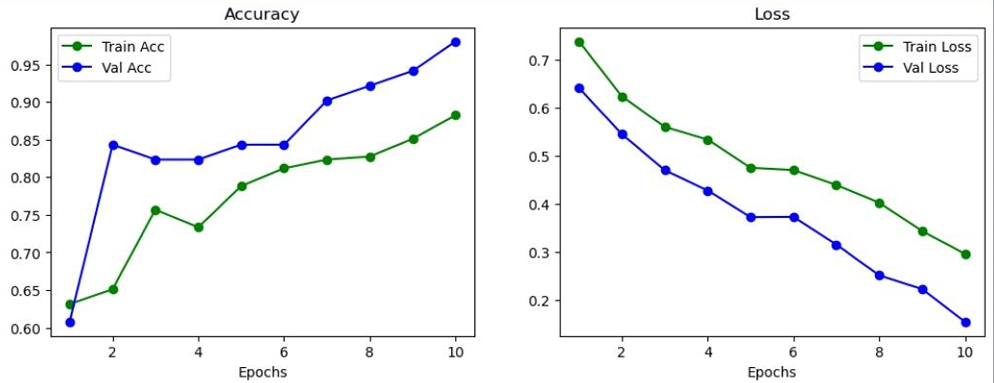
\includegraphics[width=0.96\textwidth, height=0.80\textheight,
                     keepaspectratio]{images/training-and-validation.png}
\end{frame}

% ===========================================================================
\section{Results}
% ===========================================================================

\begin{frame}{Model Performance --- Key Metrics}
  \centering
  \vspace{0.2cm}
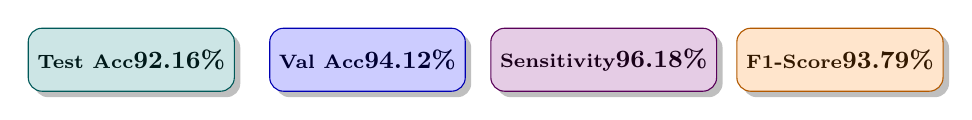
\begin{tikzpicture}
    \node[metricbox=teal,   minimum width=1.6cm, minimum height=0.8cm] (acc)  at (0,0)   {\scriptsize Test Acc\vspace{2pt}\par\small 92.16\%};
    \node[metricbox=blue,   minimum width=1.6cm, minimum height=0.8cm] (vacc) at (3.0,0) {\scriptsize Val Acc\vspace{2pt}\par\small 94.12\%};
    \node[metricbox=violet, minimum width=1.6cm, minimum height=0.8cm] (sens) at (6.0,0) {\scriptsize Sensitivity\vspace{2pt}\par\small 96.18\%};
    \node[metricbox=orange, minimum width=1.6cm, minimum height=0.8cm] (f1)   at (9.0,0) {\scriptsize F1-Score\vspace{2pt}\par\small 93.79\%};
\end{tikzpicture}

  \vspace{0.4cm}
  \renewcommand{\arraystretch}{1.2}
  {\small
  \begin{tabular}{|l|c|l|}
  \hline
  \rowcolor{black}
  \textcolor{white}{\textbf{Metric}} &
  \textcolor{white}{\textbf{Value}} &
  \textcolor{white}{\textbf{Formula / Notes}} \\
  \hline
  True Positives  (Tumour) & 151     & Correct tumour detections \\
  \hline
  True Negatives  (Normal) & 84      & Correct normal classifications \\
  \hline
  False Positives          & 14      & Normal misclassified as Tumour \\
  \hline
  False Negatives          & 6       & Tumour misclassified as Normal \\
  \hline
  Precision                & 91.52\,\% & $\text{TP}/(\text{TP}+\text{FP})$ \\
  \hline
  Specificity              & 85.71\,\% & $\text{TN}/(\text{TN}+\text{FP})$ \\
  \hline
  \end{tabular}}
\end{frame}

\begin{frame}{Confusion Matrix}
    \centering
    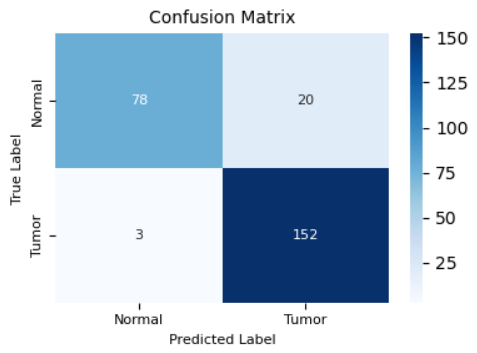
\includegraphics[width=0.96\textwidth, height=0.80\textheight,
                     keepaspectratio]{images/confussion-matrix.png}
\end{frame}

\begin{frame}{Confusion Matrix --- Clinical Interpretation}
  \begin{columns}[T]
    \column{0.50\textwidth}
    \textbf{What the numbers mean:}
    \begin{itemize}\setlength\itemsep{4pt}
        \item \textbf{151 TP:} Tumours correctly flagged for treatment
        \item \textbf{84 TN:} Healthy patients correctly cleared
        \item \textbf{14 FP:} Unnecessary follow-up scans (low risk)
        \item \textbf{6 FN:} Missed tumours --- most critical error
    \end{itemize}
    \vspace{0.3cm}
    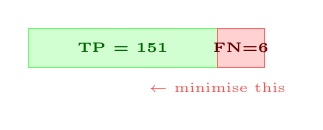
\begin{tikzpicture}
      \draw[fill=green!18, draw=green!60] (0,0) rectangle (2.4,0.5)
            node[midway, font=\tiny\bfseries, text=green!40!black]{TP = 151};
      \draw[fill=red!18,   draw=red!60]   (2.4,0) rectangle (3.0,0.5)
            node[midway, font=\tiny\bfseries, text=red!40!black]{FN=6};
      \node[font=\tiny, text=red!70, below=2pt] at (2.4,0) {$\leftarrow$ minimise this};
    \end{tikzpicture}

    \column{0.46\textwidth}
    \textbf{Clinical Context:}
    \begin{itemize}\setlength\itemsep{4pt}
        \item Sensitivity 96.18\,\% --- 96 of 100 tumours detected
        \item Suitable as a preliminary screening tool
        \item False positives trigger radiologist review (safe)
        \item False negatives bypass treatment (dangerous)
        \item Model is intentionally tuned to minimise FN
    \end{itemize}
  \end{columns}
\end{frame}

\begin{frame}{PCA Feature Space Visualisation}
    \centering
    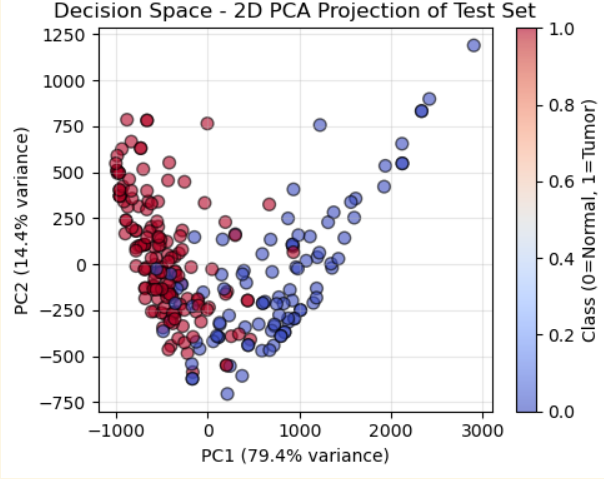
\includegraphics[width=0.96\textwidth, height=0.80\textheight,
                     keepaspectratio]{images/pca-projection-test.png}
\end{frame}

\begin{frame}{PCA --- Interpretation}
  \begin{columns}[T]
    \column{0.50\textwidth}
    \textbf{What PCA reveals:}
    \begin{itemize}\setlength\itemsep{4pt}
        \item Features extracted from penultimate Dense(256) layer
        \item 256-dimensional vectors projected to 2D
        \item PC1 explains \textbf{75.3\,\%} of variance
        \item PC2 explains \textbf{15.7\,\%} of variance
        \item Total: \textbf{90.9\,\%} variance retained
    \end{itemize}
    \column{0.46\textwidth}
    \textbf{Significance:}
    \begin{itemize}\setlength\itemsep{4pt}
        \item Clear spatial separation between classes
        \item Confirms CNN learned discriminative features
        \item Not relying on superficial pixel patterns
        \item High separability $\rightarrow$ reliable decisions
    \end{itemize}
    \vspace{0.3cm}
    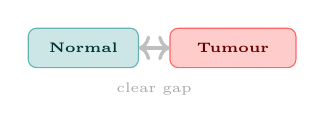
\begin{tikzpicture}
      \draw[fill=teal!20, draw=teal!60, rounded corners=3pt]
           (0,0) rectangle (1.4,0.5)
           node[midway,font=\tiny\bfseries,text=teal!40!black]{Normal};
      \draw[fill=red!20, draw=red!60, rounded corners=3pt]
           (1.8,0) rectangle (3.4,0.5)
           node[midway,font=\tiny\bfseries,text=red!40!black]{Tumour};
      \draw[very thick, gray!50, <->] (1.4,0.25)--(1.8,0.25);
      \node[font=\tiny, text=gray!70, below=2pt] at (1.6,0){clear gap};
    \end{tikzpicture}
  \end{columns}
\end{frame}

% ===========================================================================
\section{Mathematical Foundation}
% ===========================================================================

\begin{frame}{Loss Function and Optimisation}
    \textbf{Binary Cross-Entropy Loss:}
    \[
        \mathcal{L} = -\frac{1}{N}\sum_{i=1}^{N}
        \Bigl[y_i \log\hat{y}_i + (1-y_i)\log(1-\hat{y}_i)\Bigr]
    \]

    \vspace{0.2cm}
    \textbf{Adam Optimiser Update Rule:}
    \[
        \theta_{t+1} = \theta_t - \frac{\eta}{\sqrt{\hat{v}_t}+\epsilon}\,\hat{m}_t
        \quad \text{where } \eta = 0.001
    \]

    \vspace{0.25cm}
    \centering
    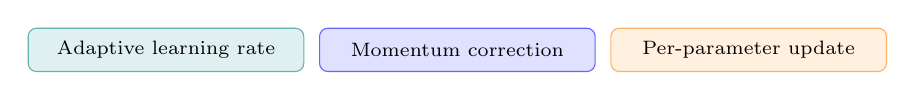
\begin{tikzpicture}
      \node[rectangle, rounded corners=3pt, draw=teal!60, fill=teal!12,
            minimum width=3.5cm, minimum height=0.55cm, font=\scriptsize]
            at (-3.7,0){Adaptive learning rate};
      \node[rectangle, rounded corners=3pt, draw=blue!60, fill=blue!12,
            minimum width=3.5cm, minimum height=0.55cm, font=\scriptsize]
            at (0,0){Momentum correction};
      \node[rectangle, rounded corners=3pt, draw=orange!60, fill=orange!12,
            minimum width=3.5cm, minimum height=0.55cm, font=\scriptsize]
            at (3.7,0){Per-parameter update};
    \end{tikzpicture}
\end{frame}

\begin{frame}{Classification Metrics}
    \textbf{Precision, Recall, F1-Score:}
    \[
        \text{Precision} = \frac{\text{TP}}{\text{TP}+\text{FP}} = 91.52\,\%
        \qquad
        \text{Recall} = \frac{\text{TP}}{\text{TP}+\text{FN}} = 96.18\,\%
    \]
    \[
        F_1 = \frac{2 \cdot \text{Precision} \cdot \text{Recall}}%
                   {\text{Precision} + \text{Recall}} = 93.79\,\%
    \]

    \vspace{0.25cm}
    \textbf{Sigmoid Output (Binary Decision):}
    \[
        \hat{y} = \sigma(z) = \frac{1}{1+e^{-z}}
        \quad \Rightarrow \quad
        \text{class} = \begin{cases}
          \text{Tumour} & \hat{y} \geq 0.5 \\
          \text{Normal} & \hat{y} < 0.5
        \end{cases}
    \]
\end{frame}

% ===========================================================================
\section{Sustainable Development Goals}
% ===========================================================================

\begin{frame}{SDG Alignment}
  \centering
  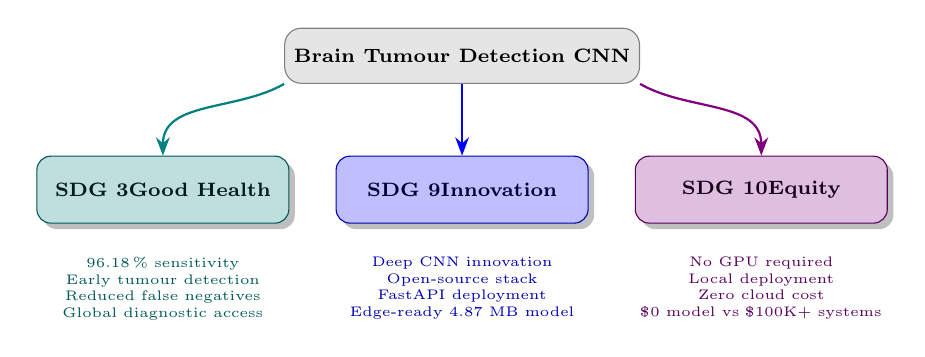
\begin{tikzpicture}[node distance=0.4cm and 0.5cm]
    \node[rectangle, rounded corners=6pt, fill=gray!20, draw=gray,
          minimum width=4.0cm, minimum height=0.7cm,
          font=\scriptsize\bfseries]
         (proj) at (3.8, 2.5){Brain Tumour Detection CNN};

    \node[sysbox=teal,   minimum width=3.2cm] (s3)  at (0,   0.8){SDG 3\\Good Health};
    \node[sysbox=blue,   minimum width=3.2cm] (s9)  at (3.8, 0.8){SDG 9\\Innovation};
    \node[sysbox=violet, minimum width=3.2cm] (s10) at (7.6, 0.8){SDG 10\\Equity};

    \draw[pipearrow, teal]  (proj.south west) to[out=210,in=90](s3.north);
    \draw[pipearrow, blue]  (proj.south)                      --(s9.north);
    \draw[pipearrow, violet](proj.south east) to[out=330,in=90](s10.north);

    \node[below=0.3cm of s3,  font=\tiny, text=teal!70!black,
          align=center, text width=3.2cm]
         {96.18\,\% sensitivity\\Early tumour detection\\Reduced false negatives\\Global diagnostic access};

    \node[below=0.3cm of s9,  font=\tiny, text=blue!70!black,
          align=center, text width=3.2cm]
         {Deep CNN innovation\\Open-source stack\\FastAPI deployment\\Edge-ready 4.87 MB model};

    \node[below=0.3cm of s10, font=\tiny, text=violet!70!black,
          align=center, text width=3.2cm]
         {No GPU required\\Local deployment\\Zero cloud cost\\\$0 model vs \$100K+ systems};
  \end{tikzpicture}
\end{frame}

% ===========================================================================
\section{Future Enhancements}
% ===========================================================================

\begin{frame}{Future Roadmap}
  \centering
  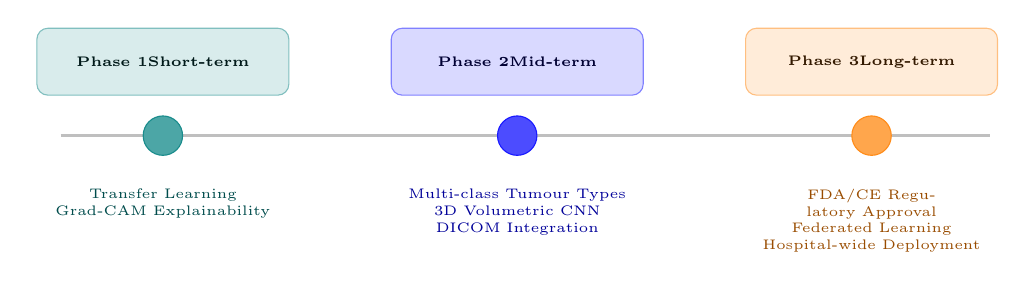
\begin{tikzpicture}
    \draw[very thick, gray!50](-0.3,0)--(11.5,0);

    \node[circle, fill=teal!70, draw=teal!90, minimum size=0.5cm,
          text=white, font=\tiny\bfseries](c1) at (1.0,0){};
    \node[rectangle, rounded corners=4pt, fill=teal!15, draw=teal!50,
          minimum width=3.2cm, minimum height=0.85cm,
          font=\tiny\bfseries, text=teal!20!black, above=0.25cm of c1]
         {Phase 1\\Short-term};
    \node[font=\tiny, text=teal!60!black, below=0.3cm of c1,
          text width=3.2cm, align=center]
         {Transfer Learning\\Grad-CAM Explainability};

    \node[circle, fill=blue!70, draw=blue!90, minimum size=0.5cm,
          text=white, font=\tiny\bfseries](c2) at (5.5,0){};
    \node[rectangle, rounded corners=4pt, fill=blue!15, draw=blue!50,
          minimum width=3.2cm, minimum height=0.85cm,
          font=\tiny\bfseries, text=blue!20!black, above=0.25cm of c2]
         {Phase 2\\Mid-term};
    \node[font=\tiny, text=blue!60!black, below=0.3cm of c2,
          text width=3.2cm, align=center]
         {Multi-class Tumour Types\\3D Volumetric CNN\\DICOM Integration};

    \node[circle, fill=orange!70, draw=orange!90, minimum size=0.5cm,
          text=white, font=\tiny\bfseries](c3) at (10.0,0){};
    \node[rectangle, rounded corners=4pt, fill=orange!15, draw=orange!50,
          minimum width=3.2cm, minimum height=0.85cm,
          font=\tiny\bfseries, text=orange!20!black, above=0.25cm of c3]
         {Phase 3\\Long-term};
    \node[font=\tiny, text=orange!60!black, below=0.3cm of c3,
          text width=3.2cm, align=center]
         {FDA/CE Regulatory Approval\\Federated Learning\\Hospital-wide Deployment};
  \end{tikzpicture}

  \vspace{0.55cm}
  \begin{columns}
    \column{0.32\textwidth}\centering
      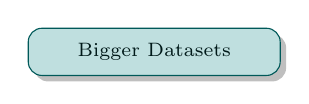
\begin{tikzpicture}
        \node[sysbox=teal, minimum width=3.2cm, minimum height=0.6cm,
              font=\scriptsize]{Bigger Datasets};
      \end{tikzpicture}
    \column{0.32\textwidth}\centering
      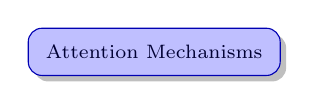
\begin{tikzpicture}
        \node[sysbox=blue, minimum width=3.2cm, minimum height=0.6cm,
              font=\scriptsize]{Attention Mechanisms};
      \end{tikzpicture}
    \column{0.32\textwidth}\centering
      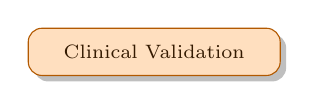
\begin{tikzpicture}
        \node[sysbox=orange, minimum width=3.2cm, minimum height=0.6cm,
              font=\scriptsize]{Clinical Validation};
      \end{tikzpicture}
  \end{columns}
\end{frame}

% ===========================================================================
\section{Conclusions}
% ===========================================================================

\begin{frame}{Key Achievements}
    \begin{columns}[T]
        \column{0.48\textwidth}
        \textbf{Technical Success:}
        \begin{itemize}\setlength\itemsep{4pt}
            \item 4-stage CNN trained from scratch
            \item 92.16\,\% test accuracy achieved
            \item 94.12\,\% validation accuracy (epoch 10)
            \item 96.18\,\% sensitivity --- only 6 FN in 157 tumours
            \item PCA confirms 90.9\,\% class separability
            \item Exported .keras model via FastAPI
        \end{itemize}
        \column{0.48\textwidth}
        \textbf{Clinical and Social Impact:}
        \begin{itemize}\setlength\itemsep{4pt}
            \item Pre-screening tool for radiologists
            \item Upstream classifier for DIP pipeline
            \item Ollama LLM chatbot for patient Q\&A
            \item Deploys without GPU or cloud
            \item Advances SDG 3, 9, and 10
        \end{itemize}
    \end{columns}

    \vspace{0.4cm}
    \centering
    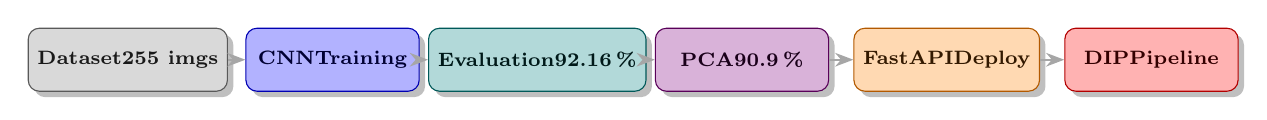
\begin{tikzpicture}
      \node[pipenode=gray,   minimum width=2.2cm, minimum height=0.8cm](r0) at (0,0)   {Dataset\\255 imgs};
      \node[pipenode=blue,   minimum width=2.2cm, minimum height=0.8cm](r1) at (2.6,0) {CNN\\Training};
      \node[pipenode=teal,   minimum width=2.2cm, minimum height=0.8cm](r2) at (5.2,0) {Evaluation\\92.16\,\%};
      \node[pipenode=violet, minimum width=2.2cm, minimum height=0.8cm](r3) at (7.8,0) {PCA\\90.9\,\%};
      \node[pipenode=orange, minimum width=2.2cm, minimum height=0.8cm](r4) at (10.4,0) {FastAPI\\Deploy};
      \node[pipenode=red,    minimum width=2.2cm, minimum height=0.8cm](r5) at (13.0,0) {DIP\\Pipeline};
      \draw[pipearrow](r0.east)--(r1.west);
      \draw[pipearrow](r1.east)--(r2.west);
      \draw[pipearrow](r2.east)--(r3.west);
      \draw[pipearrow](r3.east)--(r4.west);
      \draw[pipearrow](r4.east)--(r5.west);
    \end{tikzpicture}
\end{frame}

% ===== QUESTIONS =====
\begin{frame}{Questions?}
    \vspace{0.4cm}
    \centering
    \LARGE\textbf{Questions and Discussion}
    \vspace{0.7cm}

    \normalsize
    \begin{tabular}{ll}
        \textbf{Repository:} &
        \texttt{github.com/Muhammad-Ahmad17/cancer\_cells} \\[8pt]
        \textbf{Contact:}    &
        \texttt{muhammadahmad171105@gmail.com}              \\
    \end{tabular}

    \vspace{0.7cm}
    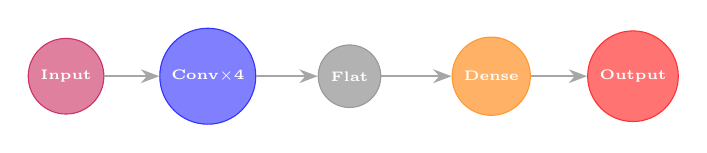
\begin{tikzpicture}
      \node[circle, fill=purple!50, draw=purple!80, minimum size=0.75cm,
            font=\tiny\bfseries, text=white](c0) at (0,0)   {Input};
      \node[circle, fill=blue!50,   draw=blue!80,   minimum size=0.75cm,
            font=\tiny\bfseries, text=white](c1) at (1.80,0){Conv\\$\times$4};
      \node[circle, fill=gray!60,   draw=gray!80,   minimum size=0.75cm,
            font=\tiny\bfseries, text=white](c2) at (3.60,0){Flat};
      \node[circle, fill=orange!60, draw=orange!80, minimum size=0.75cm,
            font=\tiny\bfseries, text=white](c3) at (5.40,0){Dense};
      \node[circle, fill=red!55,    draw=red!80,    minimum size=0.75cm,
            font=\tiny\bfseries, text=white](c4) at (7.20,0){Output};
      \draw[pipearrow](c0.east)--(c1.west);
      \draw[pipearrow](c1.east)--(c2.west);
      \draw[pipearrow](c2.east)--(c3.west);
      \draw[pipearrow](c3.east)--(c4.west);
    \end{tikzpicture}
    \vspace{0.2cm}

    \small\textit{Supervised by: \textbf{Engr. Abubakar Talha}}
\end{frame}

\end{document}